\chapter{\label{chap:intro}Introdução}

Em 2014, 54\% da população mundial vivia em áreas urbanas, de acordo com a Organização das Nações Unidas \cite{UN14}. A expectativa é que esta proporção aumente para 66\% até o ano 2050. Em números absolutos isto representa um acréscimo de 2,5 bilhões de pessoas à população urbana mundial nos próximos 35 anos. Uma das consequências da alta densidade populacional em regiões geográficas limitadas é o crescimento do modelo de verticalização na construção civil. Neste cenário, onde prédios de diversos andares se tornam presença no cotidiano da maioria da população, os elevadores passam a um papel de destaque.

Uma pesquisa realizada pela IBM no ano de 2010 em 16 cidades norte-americanas constatou que, durante 12 meses, o tempo acumulado no qual trabalhadores de escritórios\footnote{Em uma força de trabalho total de 51 milhões de trabalhadores, dos quais 12,7 milhões são usuários de elevadores diariamente \cite{IBM10}.} aguardaram por elevadores foi de 92 anos \cite{IBM10}. Em uma economia onde o salário horário médio de um trabalhador é de US\$ 24,99, o tempo de espera por elevadores representa custos de mais de US\$ 20 bilhões em média por ano \cite{BLS15}.

Além do impacto econômico existe o impacto psicológico. Trabalhadores em centros metropolitanos empreendem uma parcela significativa da sua rotina no deslocamento entre residência e local de trabalho e no caminho inverso ao final do dia. Além de gastar uma quantidade significativa de tempo no trânsito das ruas, em carros, ônibus, bicicletas e metrôs, o tempo compreendido entre aguardar o elevador e desembarcar no andar desejado está longe de ser desprezível. Em função disso, ajustam sua rotina abrindo mão de momentos de momentos de descanso ou lazer. Uma possível consequência é um aumento nos níveis de estresse e um decréscimo na qualidade de vida a médio e longo prazo. {\color{red}[BUSCAR FONTES PARA ESTE PARÁGRAFO]} % TODO: CITATIONNEEDED

\begin{figure}[htb!]
\centering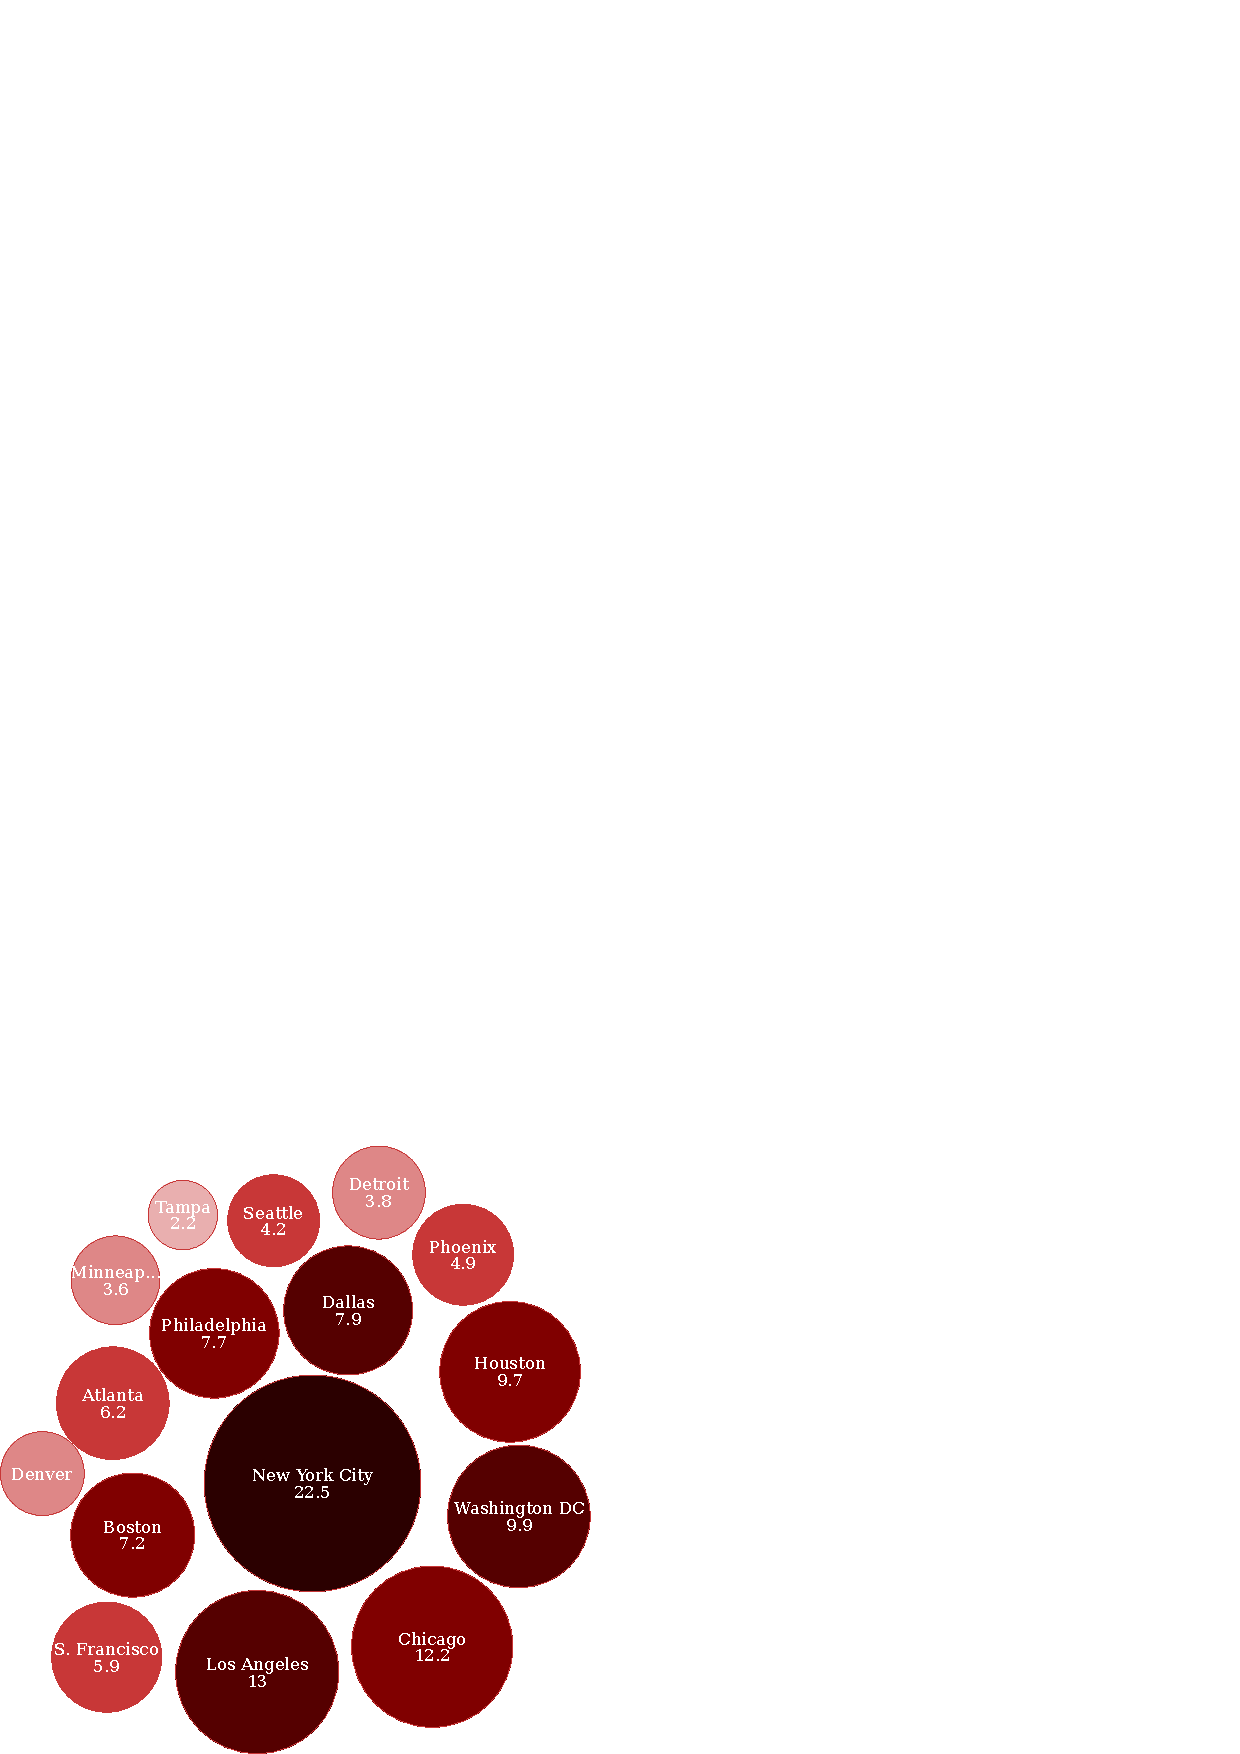
\includegraphics{img/time-cost.jpg}
\caption{\label{fig:fig1}Tempo de espera acumulado (em anos) por elevadores durante 12 meses em 16 cidades norte-americanas. Fonte: \cite{IBM10}}
\end{figure}

Neste contexto global, a indústria de elevadores possui alguns desafios: primeiro, lidar com a pressão para a redução de custos na construção civil, construindo elevadores mais baratos e eficientes, com melhorias no desempenho de transporte; segundo, competir no mercado oferecendo serviços novos, personalizados e com garantia de qualidade, visando revolucionar a maneira com que elevadores interagem e servem passageiros \cite{KOEHLEROTTIGER02}. Do ponto de vista dos passageiros, estes esperam que um elevador atenda-o imediatamente e leve-o ao seu destino o mais rápido possível. Entretanto, este problema não é de simples solução.

De fato, a tarefa de atribuir elevadores para atender chamadas minimizando tempo médio de espera é um problema NP-difícil (ou NP-hard, ou NP-complexo), conforme provado por \cite{SeKo99}. Assim sendo, para ajudar a atingir estes objetivos, fabricantes de elevadores vem estudando e implementando soluções alternativas desde meados dos anos 1980. Diversas técnicas de Inteligência Artificial foram adotadas pela indústria, como redes neurais, algoritmos genéticos, lógicas \textit{fuzzy} e, mais recentemente, sistemas multi-agentes e planejamento \cite{KOEHLEROTTIGER02}.

\section{Motivação prática}

...

\section{Testar conhecimentos}

...

\subsection{IA}

...

\subsection{Programação}

...

\section{Simulação}

...